\chapter{IoT Device Management}
In Zukunft ist eine stark ansteigende Anzahl an IoT Devices zu erwarten. Laut der International Data Corporation (IDC) dürften im Jahre 2020 in etwa 30 Milliarden Devices weltweit verbunden sein \cite{IDC15}. Unternehmen könnten potenziell mehrere Tausend Sensoren für ihre Zwecke einsetzen. Bereits bei herkömmlichen Computersystemen und Servern stellt das Management eine grosse Herausforderung dar. IoT Devices dürften potenziell in einer sehr viel grösseren Anzahl verbreitet sein als herkömmliche Geräte. Herausforderungen wie die Heterogenität, Verteilung und Security verschärfen sich mit der stetig wachsenden Anzahl an Geräten. 

IoT Devices durchleben in ihrem Lebenszyklus verschiedene Stadien. Ein Device Management Tool soll die Administration in jeder dieser Phasen Unterstützen.
\section{Device Lifecycle}
Der Lebenszyklus eines IoT Devices könnte beispielsweise aus folgenden fünf Phasen bestehen.
\begin{figure}[H]
\centering
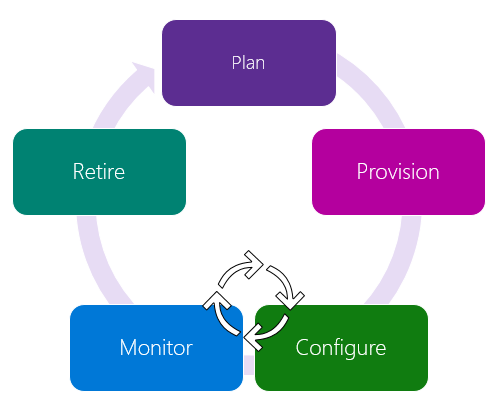
\includegraphics[scale=0.5]{images/hubdevmgmt-azure.png}
\caption{IoT Management Azure \cite{IoTMgmtAzure}}
\end{figure}
\subsubsection{Plan}
In der Planungsphase möchte man aufgrund von vorliegenden Daten eine Veränderung am System vornehmen. Um fundierte Entscheide in der Planungsphase zu ermöglichen werden Daten und Messwerte von Devices benötigt. Je einfacher diese Daten zugänglich-, respektive abfragbar sind, desto qualitativ hochwertiger und exakter kann geplant werden.
\subsubsection{Provision}
Neue Geräte müssen vor der produktiven Nutzung bereitgestellt werden. Dieser Prozess kann mehrere Personen und Aufgaben involvieren. Grundsätzlich werden neue Geräte in ein bestehendes System eingebunden oder ein komplett neues System aufgebaut.
\subsubsection{Configure}
Damit ein Device in den vorgesehenen Zustand versetzt werden kann benötigt es eine Konfiguration. Bei einer grossen Anzahl Devices empfiehlt es sich diesen Prozess bestmöglichst zu automatisieren. Dazu müssen alle Beteiligten  
\subsubsection{Monitor}
In der Monitoringphase sollen die Zustände der Devices überwacht werden. Ziel ist es, die Funktionalität und Korrektheit des angestrebten Verhalten sicherzustellen. Dies wird mittels periodischer Abfragen oder Observations sichergestellt. 
\subsubsection{Retire}
Am Ende des Lebenszyklus sollen Geräte geordnet aus dem System entfernt werden. Dabei gilt es den Prozess bestmöglich zu automatisieren und allfällige Vorschriften betreffend Datensicherheit und Datenschutz zu beachten. Andere Systeme wie das Inventar könnten ebenfalls in diesem Prozess beteiligt sein.
\section{Device Management Aufgaben}

\subsection{Provisionierung und Authentisierung}
\subsection{Konfiguration}
\subsection{Monitoring und Diagnose}
\subsubsection{Was ist Monitoring?}
Bei all den Millionen Devices ist ein Monitoring unerlässlich. Ohne ein ausgeklügeltes Monitoring kann die Überwachung von so vielen Devices sehr schnell chaotisch enden. Daher muss das Monitoring gut durchdacht sein, um sein Ziel nicht zu verfehlen. Doch was ist unser Ziel mit dem Monitoring? \newline\newline
Das Hauptziel des Monitorings ist das proaktive Überwachen der Geräte. Dadurch verringert sich nicht nur die Zeit, die benötigt wird um den Fehler zu erkennen, sondern auch die benötigte Reparaturzeit. So kann die Uptime jedes Sensors möglichst gross gehalten werden und die Produktivität steigt. Ein weiteres Ziel ist das Erkennen von Muster. So können all die gesammelten Daten zusammengefügt werden und die Muster analysiert werden. Dies führt zu einer besseren Früherkennung und auch zu einem Know-How-Gewinn. So können zukünftige Probleme besser erkannt und schneller behoben oder sogar vermieden werden.\cite{MonZiele} \newline\newline
Nun gibt es aber neue Hindernisse bei der Überwachung von IoT-Sensoren. Nicht nur, dass es eine grössere Anzahl zu überwachende Geräte gibt, sondern auch immer neue Protokolle, Geräte die sich verschieben (SmartCars) oder auch Probleme durch den noch eher jungen Entwicklungsstand gewisser Geräte. Um ein vernünftiges Monitoring im Bereich IoT bereitzustellen, muss man daher viel bedenken, was beim normalen Server oder Netzwerkmonitoring nicht wichtig war.
\subsubsection{Monitoring im IoT-Bereich}
Im Bereich IoT gibt es spezielle Anforderungen an das Monitoring. Durch die vielen Geräte und die dynamischen Netzwerke muss das Monitoring sehr Flexibel sein. Täglich werden neue Geräte eingeführt und alte entsorgt. Nicht nur der Austausch von Geräten ist mühselig, sondern auch der Standortwechsel. Die Geräte bewegen sich zum Teil und sind so in verschiedenen Netzwerken. Wenn hier kein sinnvolles System eingesetzt wird, häufen sich die fehlerhaften Meldungen und das Monitor wird ineffizient. \newline\newline
Ein weiterer wichtiger Punkt bei IoT-Geräten, ist die Team Kollaboration. Ein einzelner Mitarbeiter hat nicht die Kapazität, alleine Millionen von Sensoren zu Überwachen und zu Warten. Zusätzlich kommen noch weitere Komponenten wie Gateways, Netzwerke oder Clouddienste dazu. Um allen Bereichen ein praktikables Monitoring bereit zu stellen, benötigt man viel Know-how und ein guter Umgang mit den erhaltenen Daten. \newline\newline
\text Bei all den verschiedenen Geräten, stellt sich die Frage. Wie strikt muss die Überwachung eigentlich sein? Hier kann man das Ganze in zwei Bereiche unterteilen. Real-Time Monitoring und Non-Real-Time Monitoring. Die meisten Sensoren benötigen ganz klar kein Real-Time Monitoring. Die Sensoren wachen alle paar Minuten auf, messen die gewünschten Werte, senden diese an einen Gateway und legen sich wieder schlafen. Hier wäre ein Real-Time Monitoring nicht das richtige, da es zu vielen Fehlalarmen kommt. Bei anderen Sensoren kann dies aber sehr wohl ein wichtig sein. Bedenkt man ein Katastrophen-Überwachungssystem, dass nicht ausfallen darf, muss man ein Real-Time Monitoring einrichten. Daher ist es sehr wichtig, dies richtig abzuschätzen, um den grössten Nutzen herauszuholen. \newline\newline
Schlussendlich unterscheidet sich auch die Art der Überwachung. IoT-Monitoring ist nicht mit einem Servermonitoring gleichzustellen. Bei Serverfarmen ist die Auslastung, der verfügbare Speicher oder auch die Verfügbarkeit wichtig. Bei Sensoren sieht dies anders aus. Da die Geräte sowieso keine grosse Last bewältigen müssen, oder der Speicher nicht relevant ist, muss das Monitoring auf andere Faktoren angepasst werden. Wichtig ist daher die Verfügbarkeit der Sensoren. Spricht der Sensor immer wieder mit mir oder ist er nicht mehr Erreichbar. Oder auch die gewonnen Daten können wichtig sein. Falls zum Beispiel bei Temperaturmessungen arktische Kälte anstelle von sommerlichen Temperaturen gemessen werden, ist das sicher auch ein Indiz für Fehlverhalten.\cite{MonTypes}
\subsection{Maintenance und Update}
\subsubsection{Was versteht man unter Maintenance und Update}
Predictive Maintenance And The Industrial Internet Of Things

\subsubsection{Maintenance und Update im IoT-Bereich}



1. Greater Adoption of Predictive Maintenance
3. Accurate Performance Metrics
4. Automatic Software Upgrades
5. Recommended Repair Actions
7. Remote Assets
\cite{MaintenIoTDef}




\subsection{Security Management}
\subsubsection{Was bedeutet Security Management?}

Passwort verwaltung

Nach FCAPS
Access Logs
Security Alarms
User Access Rights



\subsubsection{Security Management im Bereich IoT}


\cite{SecOverview}
DTLS
TLS
Login


\section{}